\documentclass[tikz, border=25pt]{standalone}
\usepackage{xcolor}
\usepackage{helvet}
\renewcommand{\familydefault}{\sfdefault}
\usepackage{amsmath}
\usetikzlibrary{shapes.geometric, arrows.meta, positioning, fit, backgrounds, calc}

\definecolor{phase2bg}{HTML}{F0FDF4}
\definecolor{phase2border}{HTML}{059669}
\definecolor{optboxbg}{HTML}{D1FAE5}
\definecolor{optboxborder}{HTML}{10B981}
\definecolor{arrowgreen}{HTML}{059669}
\definecolor{textcolor}{HTML}{0F172A}

\hyphenpenalty=10000
\exhyphenpenalty=10000

\tikzset{
  stepbox/.style={
    draw=optboxborder,
    fill=optboxbg,
    line width=1.8pt,
    rounded corners=12pt,
    align=center,
    text=textcolor,
    font=\sffamily\bfseries\Large,
    inner sep=14pt,
    text width=11.5cm,
    minimum height=1.6cm
  },
  flowarrow/.style={
    -{Stealth[length=15pt, width=12pt]},
    line width=3.8pt,
    color=arrowgreen,
    shorten >= 6pt,
    shorten <= 6pt
  },
  container/.style={
    draw=phase2border,
    fill=phase2bg,
    line width=2.8pt,
    rounded corners=22pt,
    inner sep=24pt
  }
}

\begin{document}
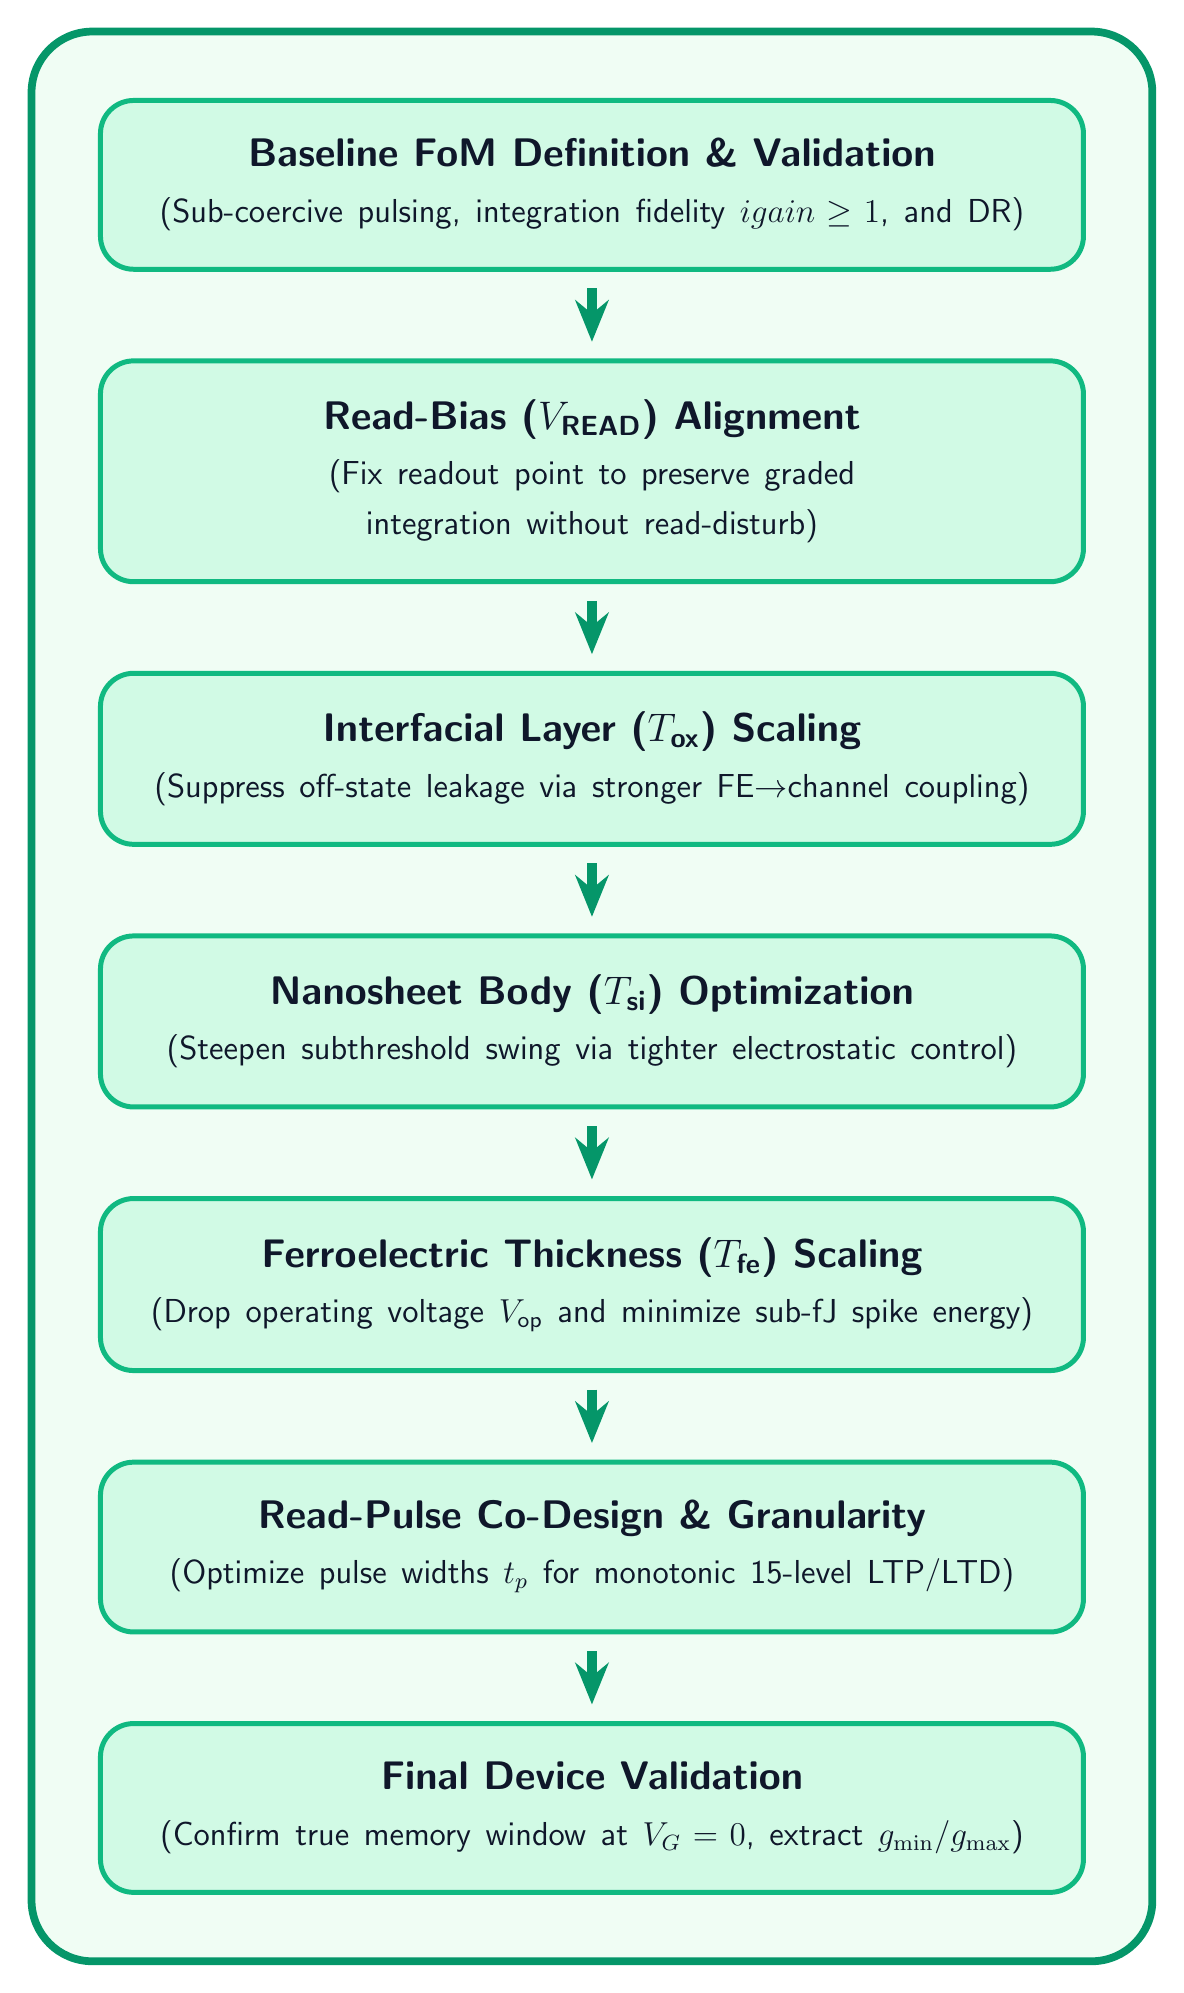
\begin{tikzpicture}[node distance=1.1cm]

  % Steps
  \node (s1) [stepbox] {Baseline FoM Definition \& Validation\\[2pt]{\large\normalfont(Sub-coercive pulsing, integration fidelity $igain \geq 1$, and DR)}};
  
  \node (s2) [stepbox, below=of s1] {Read-Bias ($V_{\text{READ}}$) Alignment\\[2pt]{\large\normalfont(Fix readout point to preserve graded integration without read-disturb)}};
  
  \node (s3) [stepbox, below=of s2] {Interfacial Layer ($T_{\text{ox}}$) Scaling\\[2pt]{\large\normalfont(Suppress off-state leakage via stronger FE$\rightarrow$channel coupling)}};
  
  \node (s4) [stepbox, below=of s3] {Nanosheet Body ($T_{\text{si}}$) Optimization\\[2pt]{\large\normalfont(Steepen subthreshold swing via tighter electrostatic control)}};
  
  \node (s5) [stepbox, below=of s4] {Ferroelectric Thickness ($T_{\text{fe}}$) Scaling\\[2pt]{\large\normalfont(Drop operating voltage $V_{\text{op}}$ and minimize sub-fJ spike energy)}};
  
  \node (s6) [stepbox, below=of s5] {Read-Pulse Co-Design \& Granularity\\[2pt]{\large\normalfont(Optimize pulse widths $t_p$ for monotonic 15-level LTP/LTD)}};
  
  \node (s7) [stepbox, below=of s6] {Final Device Validation\\[2pt]{\large\normalfont(Confirm true memory window at $V_G=0$, extract $g_{\min}/g_{\max}$)}};

  % Background container
  \begin{scope}[on background layer]
    \node (fitbox) [container, fit=(s1) (s2) (s3) (s4) (s5) (s6) (s7)] {};
  \end{scope}

  % Connectors
  \draw [flowarrow] (s1) -- (s2);
  \draw [flowarrow] (s2) -- (s3);
  \draw [flowarrow] (s3) -- (s4);
  \draw [flowarrow] (s4) -- (s5);
  \draw [flowarrow] (s5) -- (s6);
  \draw [flowarrow] (s6) -- (s7);

\end{tikzpicture}
\end{document}
